\documentclass[conference,final]{IEEEtran}

\usepackage{flushend}

\usepackage{cite}

\ifCLASSINFOpdf
  \usepackage[pdftex]{graphicx}
  \graphicspath{images/}
\else
  \usepackage[dvips]{graphicx}
  \graphicspath{images/}
\fi

\usepackage[cmex10]{amsmath}
\usepackage{amsfonts}
\usepackage{array}

\usepackage{url}

\usepackage{algorithmic, algorithm}

\usepackage{placeins}

\usepackage{tikz, pgfplots}

\usetikzlibrary{patterns}
\usetikzlibrary{external}
\tikzexternalize

\renewcommand{\algorithmicrequire}{\textbf{Input:}}
\renewcommand{\algorithmicensure}{\textbf{Output:}}

%\hyphenation{op-tical net-works semi-conduc-tor}

\begin{document}
\title{Trajectory Following for Legged Robots}

\author{ \parbox{3 in}{\centering Thomas Moulard, Florent Lamiraux\\
    LAAS-CNRS, Universit\'e de Toulouse\\
    7, avenue du Colonel Roche\\
    31077 Toulouse cedex 4, France\\
    {\tt\small thomas.moulard@laas.fr}}
  \hspace*{0.5 in}
  \parbox{3 in}{ \centering Olivier Stasse\\
    CNRS-AIST, JRL (Joint Robotics Laboratory), UMI 3218/CRT,\\
    Intelligent Systems Research Institute,\\
    AIST Central 2, Umezono 1-1-1, \\
    Tsukuba, Ibaraki 305-8568 Japan\\
    {\tt\small olivier.stasse@aist.go.jp}}
}


\maketitle


\begin{abstract}
  While robust trajectory following is a well-studied problem on
  mobile robots, the question of how to track accurately a trajectory
  on a humanoid robot remains open.

  This paper suggests a closed-loop trajectory tracking strategy
  aimed at humanoid robots. Compared to approaches from mobile
  robotics, this control scheme takes into account footsteps
  alteration, equilibrium constraints and singularities avoidance for
  humanoids. It provides a robust way to execute long and/or precise
  motion with the ability of correcting on-line preplanned
  trajectories in a very reactive manner. Results have been validated
  on the HRP-2 humanoid platform.
\end{abstract}

\begin{IEEEkeywords}
  Humanoid robots, Motion planning, Robot control
\end{IEEEkeywords}

\IEEEpeerreviewmaketitle


\section{Introduction}
%
\IEEEPARstart{F}{ollowing} a planned trajectory on a robot while
compensating execution errors has been extensively studied in the 90's
for mobile robots \cite{91icra.samson,
  98deLucaOrioloSamson}. Surprisingly, this issue has not been
explicitly addressed in the literature concerning navigation for
legged robots, although these machines are also prone to execution
errors while moving.
%
Previous experiments such as \cite{11humanoids.baudouin} illustrate
how imprecise trajectory following on a humanoid robot can be. After
executing a five meters long trajectory, the difference between the
planned and real position can reach $0.4 \textrm{m}$. Such an error
cannot be ignored anymore and invalidate the whole planning
stage. Therefore, solving this issue is crucial and will allow the
achievement of complex movements where a high precision is needed. For
instance, obstacle crossing is only feasible at the beginning of the
trajectory where the drift is not too important. This paper objective
is to provide a generic framework for robust trajectory following on a
humanoid robot.
%
One way of indirectly tackling the problem consists of regularly
replanning the motion of the robot from its current configuration to
the goal after localizing obstacles with respect to the robot. This
strategy enables the robot to be reactive to environment changes as
well as to execution errors~\cite{05humanoids.michel,
  06icra.MichelChestnut,10springer.chestnut}. On the other hand, it
requires short planning time and induces heavy CPU load. It might even
not be always be possible. Indeed most fast replanning schemes rely on
a simplified model~\cite{01icra.KajitaKanehiro} of the robot
neglecting momenta generated by the leg motions. These assumptions are
not met for small robots like Nao with a large %\cite{wikipedia.nao}
ratio of mass distributed in the legs and with a small CPU.
%
Moreover, to produce a really feasible movement, additional
constraints must be satisfied: no auto-collision should occur during
the movement for instance.
%
%
\begin{figure}[ht!]
  \begin{center}
    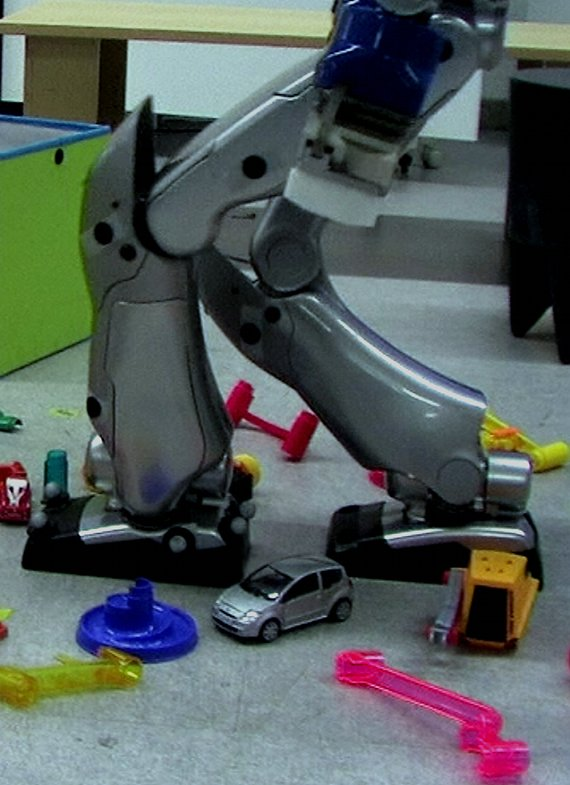
\includegraphics[width=.4\textwidth]{fig/exp2.jpg}
  \end{center}
% 4cm in x and y
  \caption{HRP-2 robot walking in a constrained
    environment. Compensating for execution errors is crucial in this
    scenario to avoid collisions. \label{fig:following}}
\end{figure}
%
%
%
For all theses reasons, validating a complex movement remains a
computationally expensive operation. Therefore, an alternative
solution to online replanning and regeneration of the walking
trajectory such as \cite{11icra.dimitrov, 10ar.herdt,
  06icra.nishiwaki, 05humanoids.michel} is the continuous deformation
of walking trajectories.  This combination of dynamic trajectories and
high probability for the robot to enter in auto-collision makes naive
correction algorithm fail which is why it is important to define a
sound framework for trajectory following.
%
%
This paper presents a ``blink of an eye'' reshaping of the trajectory
associated with a generic method to follow trajectories on a humanoid
robot. These two features together provide a way to follow a
trajectory while compensating for errors during the movement
execution. This opens many possible applications such as moving in
extremely constrained environments in a reliable manner, going to
specific places of the environment precisely, etc. Most of the state
of the art demonstration of reactive pattern generators are, in fact,
open loop trajectories with no sensors feedback. This work has been
fully integrated into the LAAS/JRL planning and control frameworks and
a motion capture system has been used to close the loop and evaluate
the execution errors.
%
This allowed HRP-2 humanoid robot to perform precise and/or long
locomotion tasks where usual open loop approaches would have drifted
so much that the task would have failed.
%
%
\section{Motivation}
%
%
This work has been motivated by the previous experimental setup
described in \cite{11humanoids.baudouin}. In this paper, fast online
replanning is used to handle environment changes. Using replanning to
cancel the drift has been considered at first but suffers from several
drawbacks. The initial idea was to accelerate replanning and consider
that there is no need to take into account the execution errors as it
can be handled by changing the robot starting position to the position
given by the localization system and regenerate the part of the
trajectory which is yet to be executed. This is difficult in practice
for several reasons. First, using the localization system as an input
of the planning component is dangerous. If the localization is
imprecise, so will be the plan. Therefore, it is required to filter
the robot position explicitly to ensure a high quality localization at
every point of time. On the opposite, as our control scheme only
modifies the next step and is bounded by a correction limit, a
low-pass filter is implicitly applied and protects the control scheme
from temporary erroneous localization. Second, if the localization is
imprecise and is near an obstacle, the estimated position may be in
collision with the obstacle. It is possible to project the robot
position outside the obstacle but additional efforts are required
during the motion planning step. To finish, even if fast replanning is
possible, randomized planning such as RRT-based methods cannot be used
safely in a real-time context as they cannot guarantee to compute a
solution within a determined time frame. In
\cite{11humanoids.baudouin}, when a replanning is required, the three
next steps cannot be modified to avoid discontinuities in the robot
trajectory. It means that the correction cannot be as reactive as it
may be necessary: the execution error may be taken into account too
late. On the opposite, the next section will demonstrate that
real-time correction is possible.
%
%
%\begin{figure}[ht!]
%  \begin{center}
%    \begin{tabular}{|c|c|c|}
%      \hline
%      \bf{Strategy} & Replanning & Correction\\
%      \hline
%      \bf{CPU usage}          & High     & Low (real-time)\\
%      \bf{Reactivity}         & Low      & High\\
%      \bf{Position filtering} & Explicit & Implicit\\
%      \hline
%    \end{tabular}
%  \end{center}
%  \caption{Comparison of replanning and online correction when
%    compensating for execution errors. \label{fig:comparison}}
%\end{figure}
%
%
%
\FloatBarrier
%
%%% Local Variables:
%%% ispell-local-dictionary: "american"
%%% LocalWords:
%%% End:

\section{Problem statement} \label{problem}
\subsection{Notation and definitions}

A \emph{robot} is a kinematic chain the configuration of which is
denoted by \mbox{$q \in \mathcal{C}$}, where $\mathcal{C}$ is the
robot configuration space.

The robot position is represented by the $x$ component, $y$ component
and yaw rotation $r_z$ of a reference body in the 3D space and is
denoted \mbox{$\mathbf{x} \in \text{SE}(2)$, $\text{SE}(2)$} the rigid
motions in the 2D space.  The height $z$, roll $r_x$ and pitch $r_y$
of the reference body are stored with the kinematic chain angles.

This reference body is often the body attached to the root of the
kinematic chain. In this paper, the position of the robot waist
defines the robot position. Therefore the robot configuration is:

\begin{equation} \label{eq:cfg}
  \begin{aligned}
    \mathbf{x} &= [x, y, r_z]\\
    \mathbf{q} &= (\mathbf{x}, [z, r_x, r_y, \mathbf{q}_{\text{int}}])
    \in \mathcal{C} = \text{SE}(2) \times \mathcal{C}_{\text{int}}
  \end{aligned}
\end{equation}



Therefore a \emph{trajectory} is a continuous function $\gamma$
associating to each point of time of the interval
\mbox{$[t_{\text{min}}, t_{\text{max}}]$} to a particular robot
configuration \mbox{$\textbf{q}(t)$}:

\begin{equation} \label{eq:traj}
  \begin{aligned}
    \gamma \colon [t_{\text{min}}, t_{\text{max}}] &\to \mathcal{C}\\
    t &\mapsto \mathbf{q}(t)
  \end{aligned}
\end{equation}


A \emph{rigid transformation} is

\begin{equation} \label{eq:rigidtrans}
  \begin{aligned}
    m \colon \text{SE}(2) \times \mathcal{C}_{\text{int}} &\to \text{SE}(2) \times \mathcal{C}_{\text{int}}\\
    (x, \mathbf{q}_{\text{int}}) &\mapsto (m . x, \mathbf{q}_{\text{int}})
  \end{aligned}
\end{equation}


An \emph{auto-collision} occurs when the robot collides with
itself. The set of all configurations in autocollision is called
\mbox{$\mathcal{Q}_{\text{col}}$}.

Walking is a sequence of one or many \emph{footstep(s)}. At the
beginning, both feet are on the floor. This phase is called
\emph{double support phase}. Then, a foot moves until it reaches a
desired position. This interval of time, until the foot lies on the
floor again is called a \emph{single support phase}. The moving foot
is the \emph{swing foot}, the static foot is the \emph{support foot}.

A footstep position is a 2D position on the plane. Steps will be
denoted by \mbox{$S \in \text{SE}(2)$}.

A walking movement can be described as a sequence of footsteps $S_i$,
\mbox{$0 \leq i \leq n^{\text{step}}$}. Step duration is constant and equal
to $T_{\text{step}}$.


\subsection{Trajectory following: from mobile robots to humanoids}


As trajectory following has been extensively studied, a direct use of
previously studied ideas such as illustrated by Fig.~\ref{fig:system}
would seem natural. However, this section will demonstrate that this
naive approach is not sufficient.


Fig.~\ref{fig:system} depicts what would be a mobile-robot closed loop
tracking system applied to a humanoid robot. The reference trajectory
$\gamma$ would be modified by a feedback provided by some external
localization system integrated to the robot and prodiving an
estimation of the robot position and orientation denoted by
$\hat{\mathbf{x}}$. From this estimation, an error is computed and
added to the original trajectory component by component using a
proportional gain, i.e.\ $k_x$, $k_y$, $k_{r_z}$ on the figure.


\begin{figure}[ht!]
  \begin{center}
    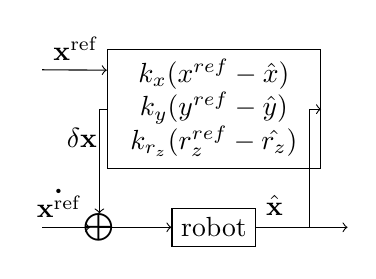
\begin{tikzpicture}[x=.40\textwidth,y=2.5cm]

      \path node (plus) at (-0.45,0) [shape=rectangle,draw,color=white]
            {\color{black} $\bigoplus$};

      \path node (robot) at (-0.15,0)
            [shape=rectangle,draw,label=3:$\hat{\mathbf{x}}$] {robot};

      \path node (errorcomp) at (-0.15,0.6)
            [shape=rectangle,draw,label=185:$\mathbf{\delta \mathbf{x}}$]
            {$\begin{array}{c} 
                k_x (x^{ref} - \hat{x})\\
                k_y (y^{ref} - \hat{y})\\
                k_{r_z} (r_z^{ref} - \hat{r_z})\end{array}$};

      \draw[-] (-0.45,0.6) -- (errorcomp.west);
      \draw[->] (-0.45,0.6) -- (-0.45,0.07);

      \draw[->] (0.1,0.6) -- (errorcomp.east);
      \draw[-] (0.1,0.6) -- (0.1,0.);
      \draw[->] (robot.east) -- (0.2,0.);

      \draw[->] (-0.45,0.) -- (robot.west);

      \draw[->] (-0.6,0.) -- (-0.474,0.) node [above left]
           {$\mathbf{\dot{\mathbf{x}^{\text{ref}}}}$};

      \draw[->] (-0.6,0.8) -- (errorcomp.160) node [above left]
           {$\mathbf{x}^{\text{ref}}$};
    \end{tikzpicture}
  \end{center}
  \caption{Naive correction system for a humanoid
    robot. $\mathbf{x}^{\text{ref}} = (x^{\text{ref}}, y^{\text{ref}},
    r_z^{\text{ref}})$, $\mathbf{\dot{x}^{\text{ref}}} =
    (\dot{x}^{\text{ref}}, \dot{y}^{\text{ref}},
    \dot{r_z}^{\text{ref}})$ and $\mathbf{\hat{x}} = (\hat{x},
    \hat{y}, \hat{r_z})$ are respectively the current planned robot
    position, velocity and position estimated by an external
    localization system. The planned control $\mathbf{\dot{x}}$ is
    rectified by summing $\delta \mathbf{x}$ a correction directly
    computed by the position error of the waist between the plan and
    the perception. \label{fig:system}}
\end{figure}


This system provides an updated trajectory of the waist taking into
account execution error through a feedback loop. As long as the
humanoid robot has at least one contact point with the floor, the
waist becomes locally fully actuated and this correction can be applied
as long as $\mathbf{q}_{\text{int}}$, the joint values are recomputed
accordingly.


\paragraph{Corrected trajectory stability}
Unlike mobile robots, humanoid robots do not have to take into account
the non-holonomic constraint which simplifies the control
scheme. However, humanoids robots must preserve equilibrium during
motion. This constraint is equivalent to the center of pressure $\mathbf{z}$
remaining in the convex hull of the contact points of the feet on the ground:


\begin{equation} \label{eq:zmp1}
  \mathbf{z} = \mathbf{x} + \frac{1}{m(\ddot{z}_c +
    g)}\left(\begin{array}{ccc} 0 &-1 &0\\1 &0 &0\end{array}\right)
    \mathbf{\dot{\textbf{L}}} - \frac{z_c}{\ddot{z}_c + g}
    \ddot{\mathbf{x}}
\end{equation}
where $z_c$ is the height of the center of mass with respect to the
ground, $m$ is the mass of the robot, $g$ is the gravity constant
\mbox{$\mathbf{x}=(x_c,y_c)$} is the projection of the center mass of
the robot on the ground and $\textbf{L}$ is the angular momentum of
the robot about the center of mass.

Naively applying a correction of the robot waist trajectory as
suggested by Fig.~\ref{fig:system} induces a perturbation of the
center of mass and thus of the center of pressure trajectories that
may violate the equilibrium constraint.

By constraining the center of mass to remain at constant height, and neglecting
variations of the angular momentum, the above equation simplifies into the
following linear relation:
\begin{equation} \label{eq:zmp2}
  \mathbf{z} = \mathbf{x}  - \frac{z_c}{g} \ddot{\mathbf{x}}
\end{equation}

Linearity implies that perturbing the center of mass trajectory by a
function of time \mbox{$\delta \mathbf{x}$} perturbates the center of
pressure trajectory according to the same relation:
\begin{equation} \label{eq:zmpperturbation}
\begin{split}
  \mathbf{z'} &= (\mathbf{x} + \mathbf{\delta x}) - \frac{z_c}{g} .
  \frac{d^2 (\mathbf{x} + \mathbf{\delta x})}{d t^2}\\
  &= \mathbf{x} - \frac{z_c}{g} \ddot{\mathbf{x}} +
  \underbrace{\mathbf{\delta x} - \frac{z_c}{g} \ddot{\mathbf{\delta
        x}}}_{\text{induced ZMP perturbation}}
\end{split}
\end{equation}

Using the simplified linear model, computing a trajectory correction is thus
the same problem as computing a dynamically balanced trajectory.

However, if the initial trajectory has been computed using the exact
multi-body model \ref{eq:zmp1}, computing a trajectory correction
using the linear model implies that approximation is performed only on
the correction and may result in trajectories of better quality from a
dynamic balance point of view.

\paragraph{Corrected trajectory singularities}
As the waist is only locally fully actuated, it is important to compute
a correction which does not introduce singularities during motion. The
presence of singularities is directly related to the relative position
of waist and contact points. However, applying directly the correction
does not trigger any modification of the contact points, i.e.\ the
footsteps. In practice, it means that as errors happen the gap between
the waist and the feet will increase and finally there is a high risk
to be unable to recompute the joints values due to the robot
mechanical limits.


From this discussion, it appears clearly that these two drawbacks make
the naive solution unsatisfactory. \textcolor{red}{Therefore,
  correcting a humanoid robot trajectory cannot be solved by
  considering it as a mobile robot: a new strategy is required to
  handle humanoids properties.}  To solve these issues, a better
control scheme allowing larger corrections and more suited to humanoid
robots will be introduced in the next section.


\FloatBarrier

%%% Local Variables:
%%% ispell-local-dictionary: "english"
%%% LocalWords:
%%% End:

\section{Closed-loop trajectory following for humanoid robots}
\label{closedloop}


This section proposes a control system for closed-loop trajectory
tracking while taking into consideration humanoid robots
specificities.


Closed-loop trajectory tracking consists in following a precomputed
trajectory while compensating for execution errors. Systems are often
composed of four components:
\begin{enumerate}
\item a trajectory generator component,
\item a localization component providing an estimation of the robot
  position,
\item an error estimation component computing the error between the
  planned position and the localization of the robot,
\item and a component reshaping the planned trajectory to compensate
  for the above error.
\end{enumerate}


The trajectory generator provides two reference data: the footstep
sequence, a set of footsteps $S_i$ such as \mbox{$0 \leq i \leq
  n^{\text{step}}$} and a whole-body trajectory \mbox{$\gamma(t \in
  [t_{\text{min}}, t_{\text{max}}]) \in \mathcal{C}$}. One advantage
of the proposed control scheme is to alter the future footstep
positions to avoid singularities. Given a known perturbation of the
footstep sequence, it is then possible to deduce the correction that
should be applied to the feet and center of mass trajectories. Once
those trajectories are computed, inverse geometry can be used to
regenerate the joints trajectories.


One iteration of the control loop is described by
Algorithm~\ref{fig:control_loop} and can be summarized as:
\begin{enumerate}
\item estimate the robot position,
\item compute the position error \mbox{$\delta \mathbf{x}$},
\item filter the error to avoid perturbing too much the initial
  trajectory and to absorb localization noise,
\item recompute the next steps positions to compensate execution
  errors and make sure the feet will land on the planned position,
\item check if the recomputed next step is feasible,
\item regenerate smooth trajectories for the feet, center of mass and
  ZMP.
\item regenerate the joints trajectories. This step is denoted by
  \mbox{$\gamma \bigoplus \delta \gamma$} in the algorithm. The
  \mbox{$\gamma \bigoplus \delta \gamma$} operation returns $\gamma$
  altered by the rigid transformation \mbox{$\delta \gamma$}. $\delta
  \gamma$ is the perturbation applied to the whole-body trajectory and
  is not directly computed as the inverse geometry is directly applied
  on the updated body positions.
\end{enumerate}


\begin{algorithm}
  \begin{algorithmic}
    \REQUIRE {$\gamma$, $t_{\text{current}}, t_{\text{next\_correction}}$}
    \ENSURE {$\gamma$, $t_{\text{current}}, t_{\text{next\_correction}}$}
    \IF {$\gamma(t_{\text{current}})$ is double support \AND
      $t_{\text{current}} \geq t_{\text{next\_correction}}$}
    \STATE estimate robot position $\mathbf{\hat{x}}$
    \STATE compute robot position error $\delta \mathbf{x}$
    \STATE compute offset $\delta \gamma$ absorbing the execution
    error $\delta \mathbf{x}$
    \IF {the perturbation $\delta \gamma$ can be applied}
    \STATE $\forall t \in [t_{\text{current}}, t_{\text{max}}],
    \gamma(t) \leftarrow \gamma(t) \bigoplus \delta \gamma(t)$
    \STATE $t_{\text{next\_correction}} \leftarrow t_{\text{current}} + 2 T_{\text{step}}$
    \ENDIF
    \ENDIF
    \STATE $\mathbf{q} \leftarrow \gamma(t_{\text{current}})$
    \STATE $t_{\text{current}} \leftarrow t_{\text{current}} + \Delta t$
  \end{algorithmic}
  \caption{Control loop at time $t_{\text{current}}$ achieving a
    closed-loop following of trajectory $\gamma$ (next correction will
    be applied at
    $t_{\text{next\_correction}}$). \label{fig:control_loop}}
\end{algorithm}


First, the robot position $\hat{\mathbf{x}}$ is perceived. The
localization system will not be detailed in this paper, see
\cite{08ijhr.stasse, 06humanoids.thompson} for instance for more
details. Although common limitations of these systems are taken into
account. The precision of the robot estimation does not decrease over
time, but can vary during the execution. This produces a noise which
may perturb the control scheme. The localization system can also fail
to provide an estimation or even sometimes provide aberrant values.

Secondly, an error $\mathbf{\delta \mathbf{x}}$ is computed by
comparing the planned and estimated position of the tracked reference
body. A threshold is applied to this value to bound the applied
corrections. In practice, it also filters out outliers and the noise
that the localization system may introduce in the system.


\begin{figure}[ht!]
  \begin{center}
    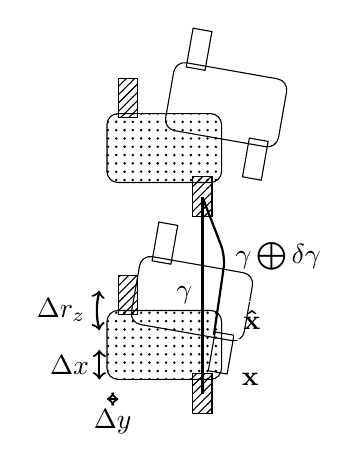
\begin{tikzpicture}[x=.40\textwidth,y=2.5cm]
      \def\w{0.3}
      \def\h{0.35}

      \def\ws{0.05}
      \def\hs{0.2}

      \def\noisex{0.01}
      \def\noisey{0.3}

      \foreach \dy in {0., 1.}
               {
                 \draw[pattern=dots,rounded corners]
                 (0.,0.25+\dy) rectangle (0.+\w,0.25+\dy+\h);

                 \draw[rotate=-10,rounded corners]
                 (\noisex,0.25+\noisey + \dy) rectangle
                 (\noisex+\w,0.25+\noisey+\dy+\h);

                 % left step planned
                 \filldraw[pattern=north east lines] (
                 0. + 0.1   * \w,
                 0.5 + \dy + 0.225 * \h)
                 rectangle (
                 0. + 0.1   * \w + \ws,
                 0.5 + \dy + 0.225 * \h + \hs);

                 % right step planned
                 \filldraw[pattern=north east lines] (
                 0. + 0.75 * \w,
                 \dy + 0.225  * \h)
                 rectangle (
                 0. + 0.75  * \w + \ws,
                 \dy + 0.225 * \h + \hs);

                 % left step real
                 \draw[rotate=-10] (
                 \noisex + 0.1   * \w,
                 0.5 + \noisey + \dy + 0.225 * \h)
                 rectangle (
                 \noisex + 0.1   * \w + \ws,
                 0.5 + \noisey + \dy + 0.225 * \h + \hs);

                 % right step real
                 \draw[rotate=-10] (
                 \noisex + 0.75 * \w,
                 \noisey + \dy + 0.225  * \h)
                 rectangle (
                 \noisex + 0.75  * \w + \ws,
                 \noisey + \dy + 0.225 * \h + \hs);
               }

               \draw[smooth,-,thick]
               (0.75 * \w + \ws/2.,\h/2.) --
               (0.75 * \w + \ws/2.,1.+\h/2.)
               node[midway,left]
               {
                 $\gamma$
               };

               \draw[smooth,rounded corners=1ex,-,thick]
               (0.75 * \w + \ws/2. + 0.03,0.15+\h/2. + 0.15) --
               (0.75 * \w + \ws/2. + 0.03 + 0.03,0.15+\h/2. + 0.15 + 0.4) --
               (0.75 * \w + \ws/2.,1.+\h/2.)
               node[at start,right]
               {
                 $\gamma \bigoplus \delta \gamma$
               };

               \draw[smooth,rounded corners=1ex,<->,thick]
               (-0.02, 0.25+0.45) --
               (-0.03, 0.25+0.35) --
               (-0.02, 0.25+0.25)
               node[at start,left]
               {
                 $\Delta r_z$
               };

               \draw[smooth,rounded corners=1ex,<->,thick]
               (-0.02, 0.25+0.) --
               (-0.02, 0.25+0.15)
               node[midway,left]
               {
                 $\Delta x$
               };

               \draw[smooth,rounded corners=1ex,<->,thick]
               (0., 0.25-0.1) --
               (0.03, 0.25-0.1)
               node[midway,below]
               {
                 $\Delta y$
               };

               \path node (txt1) at (0.075+\w,0.25+0.)
                     [shape=rectangle,draw,color=white]
                     {\color{black} $\mathbf{x}$};

               \path node (txt1) at (0.08+\w,0.25+0.3)
                     [shape=rectangle,draw,color=white]
                     {\color{black} $\mathbf{\hat{x}}$};

    \end{tikzpicture}
  \end{center}
  \caption{Correction of the next step due to a position error. Dotted
    rectangles are the planned positions $\mathbf{x}$ of the robot
    waist and feet before and after the next step. Non-dotted
    rectangles corresponds to the robot localization
    $\mathbf{\hat{x}}$. Error w.r.t to axis X, Y and yaw rotation is
    \mbox{$(\Delta x, \Delta y, \Delta r_z) = \delta \mathbf{x}$,
      $\gamma$} the reference trajectory and $\delta \gamma$ the
    corrected trajectory reaching the planned
    step. \label{fig:footstepreplan}}
\end{figure}



Then, the relative position of the next footstep w.r.t. to the current
one is changed to compensate the perceived
error. Fig.~\ref{fig:footstepreplan} illustrates this process.


From this point, smooth trajectories can be regenerated for feet and
center of mass. To ensure smoothness, the trajectory correction is
progressively applied during the next two steps. To finish, joint
values are recomputed using these new reference trajectories.



Additionally, a test is added to check that a correction can be
computed for the current time $t_{\text{current}}$. A correction can
be applied if no correction is being applied,
i.e.\ \mbox{$t_{\text{current}} \geq t_{\text{next\_correction}}$} and if the
robot is in the double support phase. Indeed starting a correction in
the middle of a step would be dangerous and starting a correction
while another correction is being applied would lead to erroneous
results.


Previous works such as \cite{04humanoids.harada, 07icra.morisawa} aim
at allowing sudden changes in the robot trajectory. The proposed
control scheme is different and aim at following as closely as
possible a preplanned trajectory.


\vspace{0.3cm}
\paragraph{Estimation of the position error}

We make the assumption that an external system provides
\mbox{$\hat{\mathbf{x}} \in \text{SE}(2)$}, an estimation of the
current robot position.

If $\mathbf{x} \in \text{SE}(2)$ is the robot planned position and
$\hat{\mathbf{x}} \in \text{SE}(2)$ the robot localization, the
position error is defined by:

\begin{equation} \label{eq:errorpos}
  \mathbf{\delta x} = \mathbf{x} . \hat{\mathbf{x}}^{-1}
\end{equation}

In Eq. (\ref{eq:errorpos}), $\mathbf{\delta x}(t)$ can be
interpreted as the planned robot position with respect to the current
robot position at time $t$. By consequence, at the beginning of the
trajectory $t_{\text{min}}$, the error is always equal to zero:

\begin{equation} \label{eq:errorpos_prop}
  \delta \mathbf{x}(t_{\text{min}}) = 0
\end{equation}

\vspace{0.3cm}
\paragraph{Footstep sequence modification}


Given a position error of the waist, it is possible to alter the
remaining steps in the footstep sequence to absorb this offset.

The purpose of this step is to take into consideration that the
previous step has not been executed correctly, leading to a different
relative position than the one which has been initially planned. To
cancel the error, the next footsteps positions will be modified
so that the robot will step in the planned locations.


The footstep positions are \mbox{$S \in
  \text{SE}(2)^{n^\text{step}}$}. Let consider $\mathbf{\delta {x}}$,
the current position error, \mbox{$S^{\text{future}} \subset S$} the
steps which have not been played yet. The footstep positions will be
changed according to the following computation:

\begin{equation} \label{eq:footstepmodif}
  \forall s \in S^{\text{future}}, s \gets \mathbf{\delta {x}} . s
\end{equation}


\vspace{0.3cm}
\paragraph{Whole-body trajectories modification}

A new placement of the next feet has been computed. It is now necessary
to modify the two feet and the center of mass trajectories
synchronously to reach the corrected foot prints.

The correction is computed by considering the simplified model
introduced in section \ref{problem}. Hence, no hypothesis is done on
the strategy used to plan the reference trajectories. One interest of
this approach is to totally dissociate the planning and correction
algorithms. To compute a small perturbation the simplified model is
sufficient. It allows extremely reactive correction without
compromising the overall trajectory quality.


The linearized inverse pendulum model allows the computation of the
center of mass trajectory $\mathbf{c}(t)$ given a ZMP trajectory
$\mathbf{z}(t)$ by solving Eq.~(\ref{eq:zmp1}). Considering $\mathbf{r}$ a
polynomial depending only of $\mathbf{z}$, $(V_x, V_y, W_x, W_y)$ free
parameters used to constrain the initial position and velocity of the
center of mass, a general following form of a polynomial center of
mass trajectory is:

\begin{equation} \label{eq:zmpsol}
  \mathbf{c}(t) = \cosh(\sqrt{\frac{g}{z_c}}.t) . \mathbf{V} + \sinh(\sqrt{\frac{g}{z_c}}.t) . \mathbf{W} + \mathbf{r}(t)
\end{equation}

Given the formulation in Eq.~(\ref{eq:zmpsol}), it is possible to
continuously modify the center of mass trajectory to make it follow
\mbox{$\bar{\mathbf{z}}(t)$} the corrected trajectory. This new
trajectory can be expressed as the sum of two polynomials:

\begin{equation} \label{eq:zmpsolcor}
  \bar{\mathbf{c}}(t) = \cosh(\sqrt{\frac{g}{z_c}}.t) . \mathbf{V} +
  \sinh(\sqrt{\frac{g}{z_c}}.t) . \mathbf{W} + \mathbf{r}(t) + \mathbf{\Delta}(t)
\end{equation}

To apply smoothly the correction from $t_1$ to $t_2$, several
constraints expressed in Eq.~\ref{eq:cst} have to be respected.
$\delta \mathbf{x}_x$ and $\delta \mathbf{x}_y$ are respectively the
$x$ and $y$ components of the 2d rigid transformation $\delta
\mathbf{x}$.

\begin{equation}
\begin{aligned}
  \mathbf{\Delta}(t_1) &= 0\\
  \mathbf{\Delta}(t_2) &= \left(
  \begin{array}{c}
    \delta \mathbf{x}_x \\
    \delta \mathbf{x}_y
  \end{array}
  \right)\\
  \frac{\partial \mathbf{\Delta}}{\partial t}(t_1) = \frac{\partial
    \mathbf{\Delta}}{\partial t}(t_2) &= 0
\end{aligned}
\label{eq:cst}
\end{equation}

\begin{figure}[ht!]
  \begin{center}

    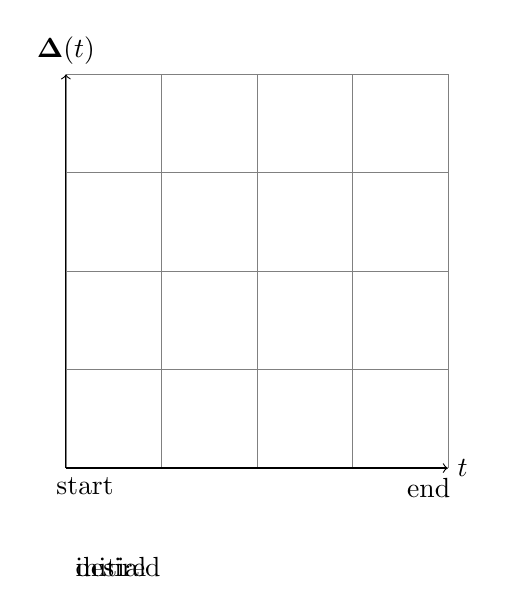
\begin{tikzpicture}[x=.40\textwidth,y=2.5cm]
      \def\xmin{0.}
      \def\xmax{1.}
      \def\ymin{0.5}
      \def\ymax{2.5}

      % grid
      \draw[style=help lines, ystep=.5, xstep=.25] (\xmin,\ymin) grid
      (\xmax,\ymax);

      % axes
      \draw[->] (\xmin,\ymin) -- (\xmax,\ymin) node[right] {$t$};
      \draw[->] (\xmin,\ymin) -- (\xmin,\ymax) node[above]
           {$\mathbf{\Delta}(t)$};

      % xticks and yticks
      \node at (0.05, \ymin) [below] {start};
      \node at (0.95, \ymin) [below] {end};

      \draw[color=black, domain=\xmin:\xmax] plot[id=cur]
      function{1} node [right] {initial};

      \draw[color=black, domain=\xmin:\xmax] plot[id=des]
      function{2} node [right] {desired};

      \draw[color=black, domain=\xmin:\xmax] plot[id=trans]
      function{-2. * x * x * x + 3 * x * x + 1} node [below] {};

    \end{tikzpicture}
  \end{center}
  \caption{Polynomial curve $\mathbf{\Delta}(t)$ providing a smooth
    transition between feet and center of mass
    trajectories. \label{fig:transition}}
\end{figure}

These four constraints determine the polynomial four parameters
leading to the curve illustrated by Fig.~\ref{fig:transition}.


\begin{figure*}[ht!]
  \begin{center}
    \begin{tikzpicture}
      \begin{axis}[
          legend style={at={(1.5,1)}, anchor=north},
          xlabel=time ($\mathrm{s}$),
          ylabel=$x$ position ($\mathrm{m}$),
          no markers
          ]

        \addplot[
          red,
          dashed
        ] table[
          x expr=(\thisrowno{0}-0)*0.005
        ] {dat/feet_follower_feet-follower-com.dat};
        \addlegendentry{center of mass}
        \addplot[
          red,
        ] table[
          x expr=(\thisrowno{0}-0)*0.005,
          y expr=\thisrowno{1}-0.
        ] {dat/feet_follower_correction-com.dat};
        \addlegendentry{center of mass (corrected)}

        \addplot[
          blue,
          dashed
        ] table[
          x index=0,
          y index=4,
          x expr=(\thisrowno{0}-0)*0.005
        ] {dat/feet_follower_feet-follower-left-ankle.dat};
        \addlegendentry{left foot}
        \addplot[
          blue
        ] table[
          x index=0,
          y index=4,
          x expr=(\thisrowno{0}-0)*0.005,
          y expr=\thisrowno{4}-0.
        ] {dat/feet_follower_correction-left-ankle.dat};
        \addlegendentry{left foot (corrected)}

        \addplot[
          green,
          dashed
        ] table[
          x index=0,
          y index=4,
          x expr=(\thisrowno{0}-0)*0.005
        ] {dat/feet_follower_feet-follower-right-ankle.dat};
        \addlegendentry{right foot}
        \addplot[
          green
        ] table[
          x index=0,
          y index=4,
          x expr=(\thisrowno{0}-0)*0.005,
          y expr=\thisrowno{4}-0.
        ] {dat/feet_follower_correction-right-ankle.dat};
        \addlegendentry{right foot (corrected)}
      \end{axis}
    \end{tikzpicture}
  \end{center}
  \caption{Evolution, during two steps, of the $x$ position of the
    center of mass and left foot. Solid curve depicts a step a $0.3
    \mathrm{m}$ forward. Dashed curve depicts this step with a
    correction of $0.05 \mathrm{m}$ in the forward
    direction. \label{fig:traj}}
\end{figure*}


This reshapes the center of mass trajectory by taking advantage of the
linear formulation of the simplified model. Additionally, the feet
trajectories are modified to reach the corrected positions at the end
of the step. The smooth correction is also obtained by using a third
degree polynomial with similar constraints: initial position remains
as before, the goal position must fit the corrected position and the
velocity of the correction is equal to zero at the beginning and the
end of the transition. Fig.~\ref{fig:traj} compares resulting
trajectories before and after the correction.


These three corrections must be executed in the correct order: as
stated before a correction is computed during a double support phase
and applied during the next two steps. We will make the assumption,
without any loss of generality, that the next flying foot is the left
one. In that case the correction of the left foot is progressively
applied during the single support phase. During the ZMP shift of this
step, the center of mass correction is also applied. Then, during the
next step, the correction of the right foot is applied. The timeline
of the correction is illustrated by Fig.~\ref{fig:traj}.


\vspace{0.3cm}
\paragraph{Error thresholding and new step feasibility}


Correction does not compromise the robot stability. However, any
correction is not feasible due to the robot mechanical limits and
auto-collision. Therefore, it is important to bound corrections in
order to avoid producing infeasible steps. It is also important to
validate new steps w.r.t to auto-collision.


The base hypothesis is that the reference trajectory which has been
computed off-line is safe i.e.\ stable and without any
auto-collision. By consequence, the goal is to determine how much this
initial trajectory can be modified without compromising its safety.

First, a maximum error has been determined empirically. The maximum
lateral perturbation is $\pm 0.04 \mathrm{m}$ , the maximum forward
perturbation $\pm 0.05 \mathrm{m}$ and the maximum angular
perturbation is $\pm 0.1 \mathrm{rad}$ every two steps.

\begin{figure}[ht!]
  \begin{center}
    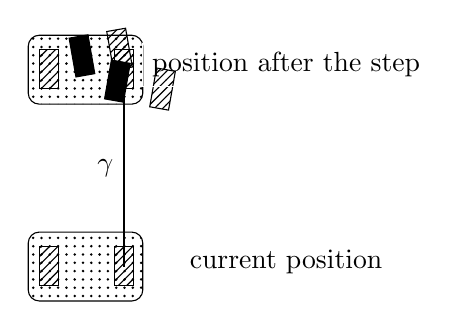
\begin{tikzpicture}[x=.40\textwidth,y=2.5cm]
      \def\w{0.3}
      \def\h{0.35}

      \def\ws{0.05}
      \def\hs{0.2}

      \def\noisex{0.01}
      \def\noisey{0.3}

      % left step planned
      \filldraw[pattern=north east lines] (
      0. + 0.1   * \w,
      0. + 0.225 * \h)
      rectangle (
      0. + 0.1   * \w + \ws,
      0. + 0.225 * \h + \hs);
      \filldraw[pattern=north east lines] (
      0. + 0.1   * \w,
      1. + 0.225 * \h)
      rectangle (
      0. + 0.1   * \w + \ws,
      1. + 0.225 * \h + \hs);


      % right step planned
      \filldraw[pattern=north east lines] (
      0. + 0.75 * \w,
      0. + 0.225  * \h)
      rectangle (
      0. + 0.75  * \w + \ws,
      0. + 0.225 * \h + \hs);

      \filldraw[pattern=north east lines] (
      0. + 0.75 * \w,
      1. + 0.225  * \h)
      rectangle (
      0. + 0.75  * \w + \ws,
      1. + 0.225 * \h + \hs);


      \foreach \dy in {0., 1.}
               {
                 \draw[pattern=dots,rounded corners] (0.,\dy)
                 rectangle (0.+\w,\dy+\h);
               }

               % valid 1
               \filldraw[pattern=north east lines,rotate=-10] (
               0. + 0.75 * \w,
               1. + 0.225  * \h)
               rectangle (
               0. + 0.75  * \w + \ws,
               1. + 0.225 * \h + \hs);

               % valid 2
               \filldraw[pattern=north east lines,rotate=10] (
               0. + 0.75 * \w + 0.1,
               1. + 0.225  * \h)
               rectangle (
               0. + 0.75  * \w + \ws + 0.1,
               1. + 0.225 * \h + \hs);


               % invalid 1
               \filldraw[color=black,rotate=10] (
               0. + 0.75 * \w,
               1. + 0.225  * \h)
               rectangle (
               0. + 0.75  * \w + \ws,
               1. + 0.225 * \h + \hs);

               % invalid 2
               \filldraw[color=black,rotate=-10] (
               0. + 0.75 * \w - 0.12,
               1. + 0.225  * \h)
               rectangle (
               0. + 0.75  * \w + \ws - 0.12,
               1. + 0.225 * \h + \hs);

               % arrow
               \draw[smooth,-,thick]
               (0.75 * \w + \ws/2.,\h/2.) --
               (0.75 * \w + \ws/2.,1.+\h/2.)
               node[midway,left]
               {
                 $\gamma$
               };

               \path node (txt1) at (0.375+\w,0.2)
                     [shape=rectangle,draw,color=white]
                     {\color{black} current position};

               \path node (txt1) at (0.375+\w,1.2)
                     [shape=rectangle,draw,color=white]
                     {\color{black} position after the step};
    \end{tikzpicture}
  \end{center}
  \caption{Validation of the recomputed next step. Waist position is
    symbolized by dotted rectangle, valid steps by hashed rectangles
    and invalid steps by black rectangles.
    \label{fig:stepvalid}}
\end{figure}


\begin{figure*}[!t]
  \begin{center}
    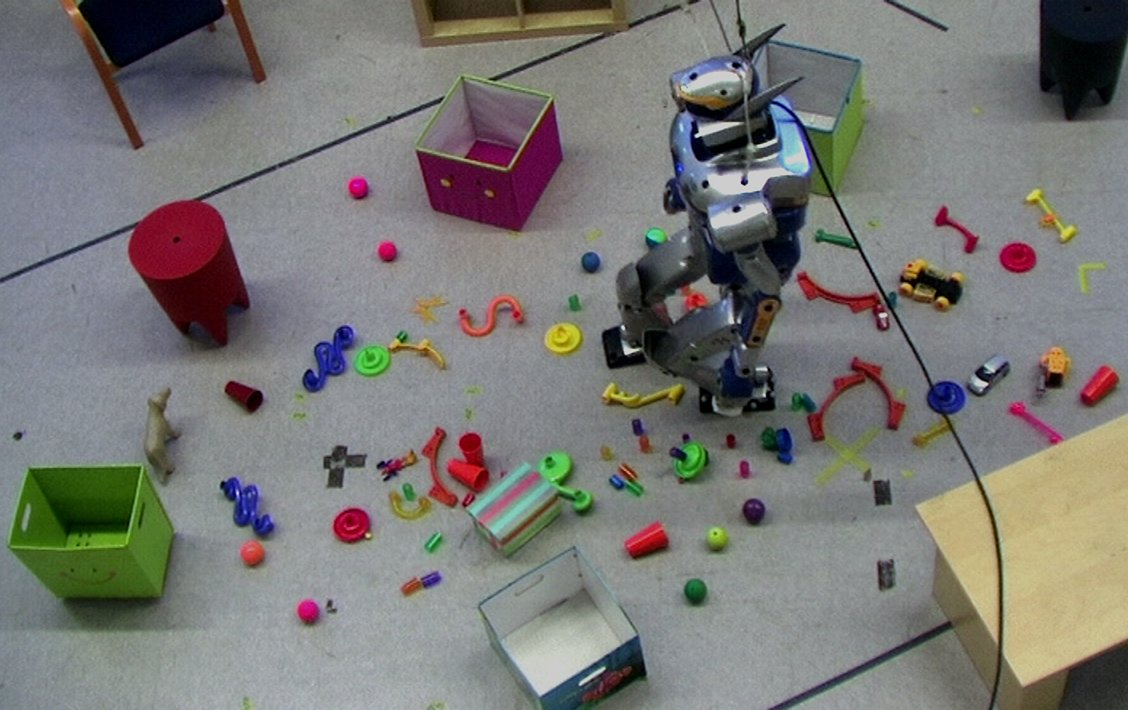
\includegraphics[width=0.85\textwidth]{fig/demo.jpg}
  \end{center}
  \caption{HRP-2 walking in a cluttered environment while avoiding
    obstacles. The final position is reached with a precision of $\pm
    3\mathrm{cm}$. The final error is the consequence of both noise in
    the robot position estimation and drifts in the two last steps
    which happen too late to be not compensated. \label{fig:scenario}}
\end{figure*}



Secondly, the new step is validated. The decision is based on the
relative movement of the first corrected foot. Let consider that, for
instance, the next moving foot is the left one. The original left foot
position is \mbox{$s \in \text{SE}(2)$}, the new corrected left foot
position is \mbox{$s' \in \text{SE}(2)$}. The relative position of the
original and new foot is computed. If the $y$ component of the result
is positive, the new step is accepted. In practice, it means that the
step is ``pushed'' away and will not induce an auto-collision. On the
opposite, with the right foot, the step is accepted if the $y$
component is negative.


If a correction is invalidated, another one is computed during the
next double support phase. In practice, the estimated error during the
next step will be close to the current estimation, in particular the
sign (i.e. direction) of the error will remain the same. As the flying
foot will change the delayed correction has a high probability of
being accepted.


This naive system has been empirically validated. However, it prevents
some valid corrected steps. In the future, this will be replaced by a
fast on-line steps validation algorithm described by
\cite{10icra.perrin}. This algorithm provides fast step validation by
precomputing feasibility regions offline. This will provide a sound
and very fast method as the validity checking will be equivalent to
reading a value in memory.

\FloatBarrier

%%% Local Variables:
%%% ispell-local-dictionary: "english"
%%% LocalWords:
%%% End:

\section{Experimental results}
\label{exp}


\textcolor{red}{SECTION REECRITE POUR ICRA}


The proposed method has been validated on HRP-2 using the following
scenarii: the robot executes a long trajectory in an environment
cluttered by obstacles located along the robot path. The followed path
is a $6\text{x}4 \mathrm{m}$ square such as the position ends at its
starting point.

This setup demonstrates that the execution using this control scheme
is precise and reliable. The robot reaches its goal position with an
error of a few centimeters whereas open loop control schemes is off by
more than a meter. Moreover, the control scheme is reliable: it takes
more than a minute for the robot to reach its goal point. During that
time, the localization precision can change, the robot position can be
lost, \ldots The control scheme is designed to be robust toward these
situations as illustrated by the video.


This experiment uses the pattern generator described by
\cite{10icra.perrin} and the stack of tasks formalism
\cite{09icar.mansard} to implement the control scheme. The pattern
generator provides reference trajectories for the center of mass and
the feet. Trajectory following tasks for these particular bodies are
then inserted into the control framework. The solver will then realize
implicitly the inverse geometry computations required to recompute the
whole-body trajectory and simplifies the actual control scheme.


\begin{figure}[ht!]
  \begin{center}
    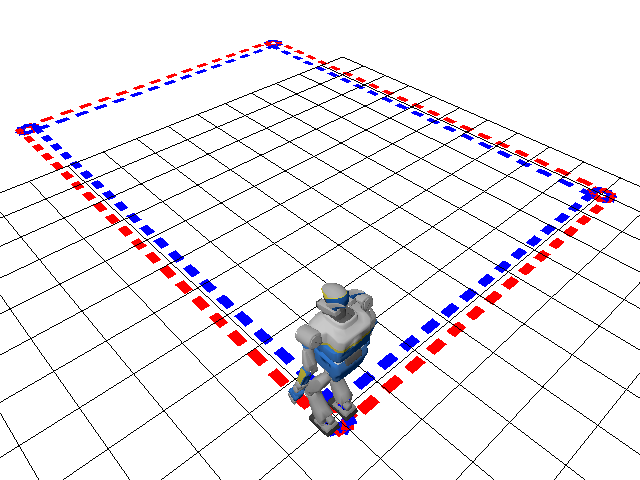
\includegraphics[width=0.45\textwidth]{fig/demo.png}
  \end{center}
  \caption{HRP-2 experiment scenario. The robot position is both
    its starting and final position. \label{fig:scenario}}
\end{figure}


Fig.~\ref{fig:following} illustrates the experiment on the real
robot. This experiment video is available on the
web\footnote{\mbox{\url{http://homepages.laas.fr/tmoulard/video/11icra-tmoulard.mp4}}}. Fig.~\ref{fig:scenario}
provides an overview of the scenario: the rectangle on the left
symbolizes the initial position and the rectangle on the right the
final position.


\begin{figure}[ht!]
  \begin{center}
    \begin{tabular}{|c|c|c|}
      \hline
      \bf{Strategy} & Replanning & Correction\\
      \hline
      \bf{CPU usage}          & High     & Low (real-time)\\
      \bf{Reactivity}         & Low      & High\\
      \bf{Position filtering} & Explicit & Implicit\\
      \hline
    \end{tabular}
  \end{center}
  \caption{Comparison of replanning and online correction when
    compensating for execution errors. \label{fig:comparison}}
\end{figure}


This work has been motivated by the previous experimental setup
described in \cite{11humanoids.baudouin}. In this paper, fast online
replanning is used to handle changes in the environment. Using
replanning to absorb the drift has been considered at first but
suffers from several drawbacks. The initial idea by using replanning
is stating that if the planning can be accelerated enough, there is no
need to take into account the execution errors as it can be handled by
changing the robot starting position to its real one instead of the
planned one and regenerating the trajectory which is yet to be
executed. This is difficult in practice for several reasons. First
using the localization system as an input of the planning component is
dangerous. If the localization is bad, so will be the plan. Therefore,
it is required to filter the robot position explicitly to ensure a
high quality localization at every point of time. On the opposite, as
our control scheme only modifies the next step and is bounded by a
correction limit, a low-pass filter is implicitly applied and
protects the control scheme from temporary erroneous
localization. Second, if the localization is imprecise and is near an
obstacle, the estimated position may be in collision with the
obstacle. Even if this is possible to project the position outside of
the obstacle, this additional step renders the replanning harder to
implement and understand. To finish, even if fast replanning is
possible, random planning such as RRT-based methods cannot be used
efficiently in a real-time context. An heuristic has been defined in
\cite{11humanoids.baudouin} indicating that when a replanning starts,
it starts three steps after the current position so that there is a
high probability that the planning ends before the robot executes
this step. It means that the correction will not be reactive and that
it may be too late when the correction is taken into account.  On the
opposite, this control scheme could provide correction at each
iteration of the control loop and could even modify the trajectory of
the swinging foot during a step. This has not been implemented as the
current strategy already provides satisfying results but it would
definitely be an interesting enhancement for a future work.


\FloatBarrier

%%% Local Variables:
%%% ispell-local-dictionary: "american"
%%% LocalWords:
%%% End:

\section{Future work and conclusion}
%
%
This paper has discussed the difference between closed-loop trajectory
tracking on a mobile robot and on a humanoid
robot. Section~\ref{problem} demonstrates that even if this problem
may seem simple, a direct use of the mobile robots control schemes is
not realistic.  Section~\ref{closedloop} suggests a new strategy which
takes into consideration the humanoid robot specificities, in
particular the need to alter contact points.
%
%
Section~\ref{exp} provides an illustration of an experiment where the
HRP-2 robot follows a trajectory and achieve a result which would be
impossible using an open loop scheme, validating the proposed
approach.
%
%
However, additional work is needed to enhance this strategy: the
heuristic step validation should be replaced by a better criteria and
maintaining a precise localization during a long movement is still a
problem. Additionally, more complex movements should be planned and
executed to validate the generality of this approach.
%
%%% Local Variables:
%%% ispell-local-dictionary: "american"
%%% LocalWords:
%%% End:


%\vfill\break

\section*{Acknowledgment}

This work has been supported by the R-BLINK project,
ANR-08-JCJC-0075-01.

%\nocite{*}
\bibliographystyle{latex/IEEEtran}
\bibliography{IEEEabrv.bib,11icra-tmoulard.bib}

\end{document}

%%% Local Variables:
%%% ispell-local-dictionary: "english"
%%% LocalWords:
%%% End:

%%% 11humanoids-tmoulard.tex ends here


